\documentclass[11  pt]{exam} 
\usepackage[lmargin=1in,rmargin=1.75in,bmargin=1in,tmargin=1in]{geometry}  


% For hyperlinking everything
\usepackage{hyperref}
\hypersetup{
	colorlinks=true, %set true if you want colored links
	linktoc=all,     %set to all if you want both sections and subsections linked
	linkcolor=blue,  %choose some color if you want links to stand out
}


\usepackage[latin1]{inputenc}
\usepackage{amsmath}
\usepackage{mathrsfs}  
\usepackage{amsfonts}
\usepackage{amssymb}
\usepackage{graphicx}
\usepackage{subfig}
\usepackage{caption}
\usepackage{algorithm}
%\usepackage{algcompatible}
%\usepackage{algorithmicx}
\usepackage{algpseudocode}

\usepackage{titlesec}
\titleformat{\section}{\fontfamily{lmss}\fontsize{14}{15}\bfseries}{\thesection}{1em}{}
\titleformat{\subsection}{\fontfamily{lmss}\fontsize{12}{15}\bfseries}{\thesubsection}{1em}{}




\usepackage{amsthm}

\newtheoremstyle{noit}
{10pt}% <Space above>
{10pt}% <Space below>
{}% <Body font>
{}% <Indent amount>
{\bfseries}% <Theorem head font>
{.}% <Punctuation after theorem head>
{.5em}% <Space after theorem headi>
{}% <Theorem head spec (can be left empty, meaning `normal')>

\newtheoremstyle{example}
{10pt}% <Space above>
{10pt}% <Space below>
{}% <Body font>
{20pt}% <Indent amount>
{\bfseries}% <Theorem head font>
{.}% <Punctuation after theorem head>
{.5em}% <Space after theorem headi>
{}% <Theorem head spec (can be left empty, meaning `normal')>


\newtheoremstyle{indented}{20pt}{20pt}{\addtolength{\leftskip}{2.5em}}{}{\bfseries}{.}{.5em}{}


\newtheorem{theorem}{Theorem}
\numberwithin{theorem}{section}
\newtheorem{lemma}[theorem]{Lemma}
\newtheorem{corollary}[theorem]{Corollary}
\newtheorem{observation}{Observation}
%\numberwithin{observation}{section}
%\numberwithin{definition}{section}
\newtheorem{conjecture}{Conjecture}
\newtheorem{Qu}{Question}
\newcommand{\QU}{\begin{Qu}\normalfont}

\theoremstyle{noit}
\newtheorem{fact}{Fact}
\newtheorem{definition}{Definition}

\theoremstyle{indented}
\newtheorem{example}{Example}

\theoremstyle{indented}
\newtheorem{problem}{Problem}


%\newenvironment{proof}{\noindent{\bf Proof:} \hspace*{1em}}{
%    \hspace*{\fill} $\Box$ }
%\newenvironment{proof_of}[1]{\noindent {\bf Proof of #1:}
%    \hspace*{1em} }{\hspace*{\fill} $\Box$ }
%\newenvironment{proof_claim}{\begin{quotation} \noindent}{
%    \hspace*{\fill} $\diamond$ \end{quotation}}
\newcommand{\vs}[1]{\vspace{#1}}

\newcommand{\lecture}[2]{
 \noindent
\begin{center}
	\framebox{
		\vbox{
			\hbox to 5.78in { {\bf CSCE 411: Design and Analysis of Algorithms} \hfill  }
			\vspace{2mm}
			\hbox to 5.78in { {\Large \hfill Lecture #1\hfill} }
			\vspace{2mm}
			\hbox to 5.78in { {\it Date: #2 \hfill Lecturer: Nate Veldt} }
		}
	}
\end{center}
\vspace*{4mm}
}


\newcommand{\hw}[2]{
	\noindent
	\begin{center}
		\framebox{
			\vbox{
				\hbox to 5.78in { {\bf CSCE 411: Design and Analysis of Algorithms} \hfill  }
				\vspace{2mm}
				\hbox to 5.78in { {\Large \hfill Homework #1\hfill} }
				\vspace{2mm}
				\hbox to 5.78in { {\it Due date: #2 \hfil} }
			}
		}
	\end{center}
	\vspace*{4mm}
}



\newcommand{\under}[1]{\underline{\hspace{#1}}}
\setlength{\parindent}{0em}

%\usepackage[tagged]{accessibility}

% Graph terms
\newcommand{\vol}{\textbf{vol}}
\newcommand{\cut}{\textbf{cut}}


% Matrices
\newcommand{\mA}{\textbf{A}}
\newcommand{\mB}{\textbf{B}}

% vectors
\newcommand{\ve}{\textbf{e}}
\newcommand{\vx}{\textbf{x}}


% Other
\newcommand{\calN}{\mathcal{N}}

\usepackage{mathtools}
\DeclarePairedDelimiter\ceil{\lceil}{\rceil}
\DeclarePairedDelimiter\floor{\lfloor}{\rfloor}


\newcommand*{\aitem}{ \item[{
\includegraphics[width=0.8cm,height=0.5cm]{../../Lectures/figures/A}} ]  }
\newcommand*{\bitem}{ \item[{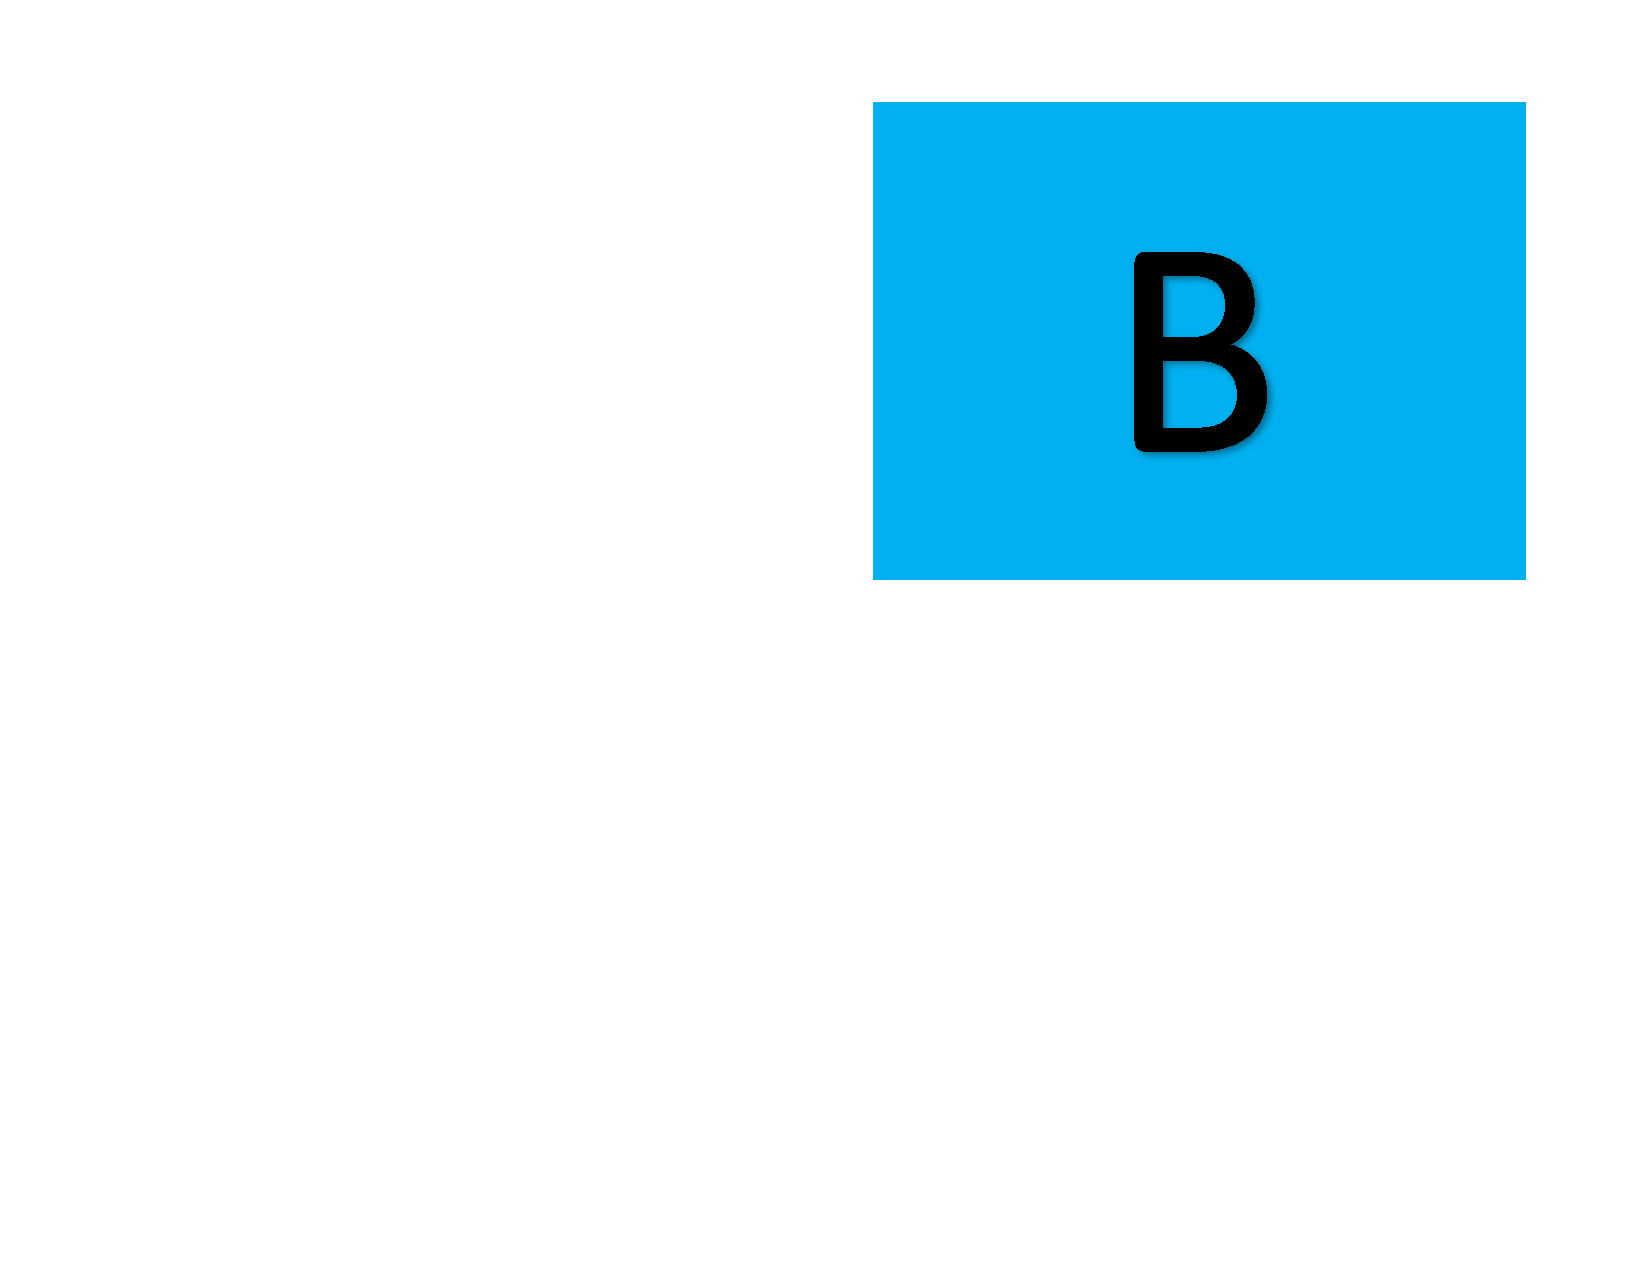
\includegraphics[width=0.8cm,height=0.5cm]{../../Lectures/figures/B}} ]  }
\newcommand*{\citem}{ \item[{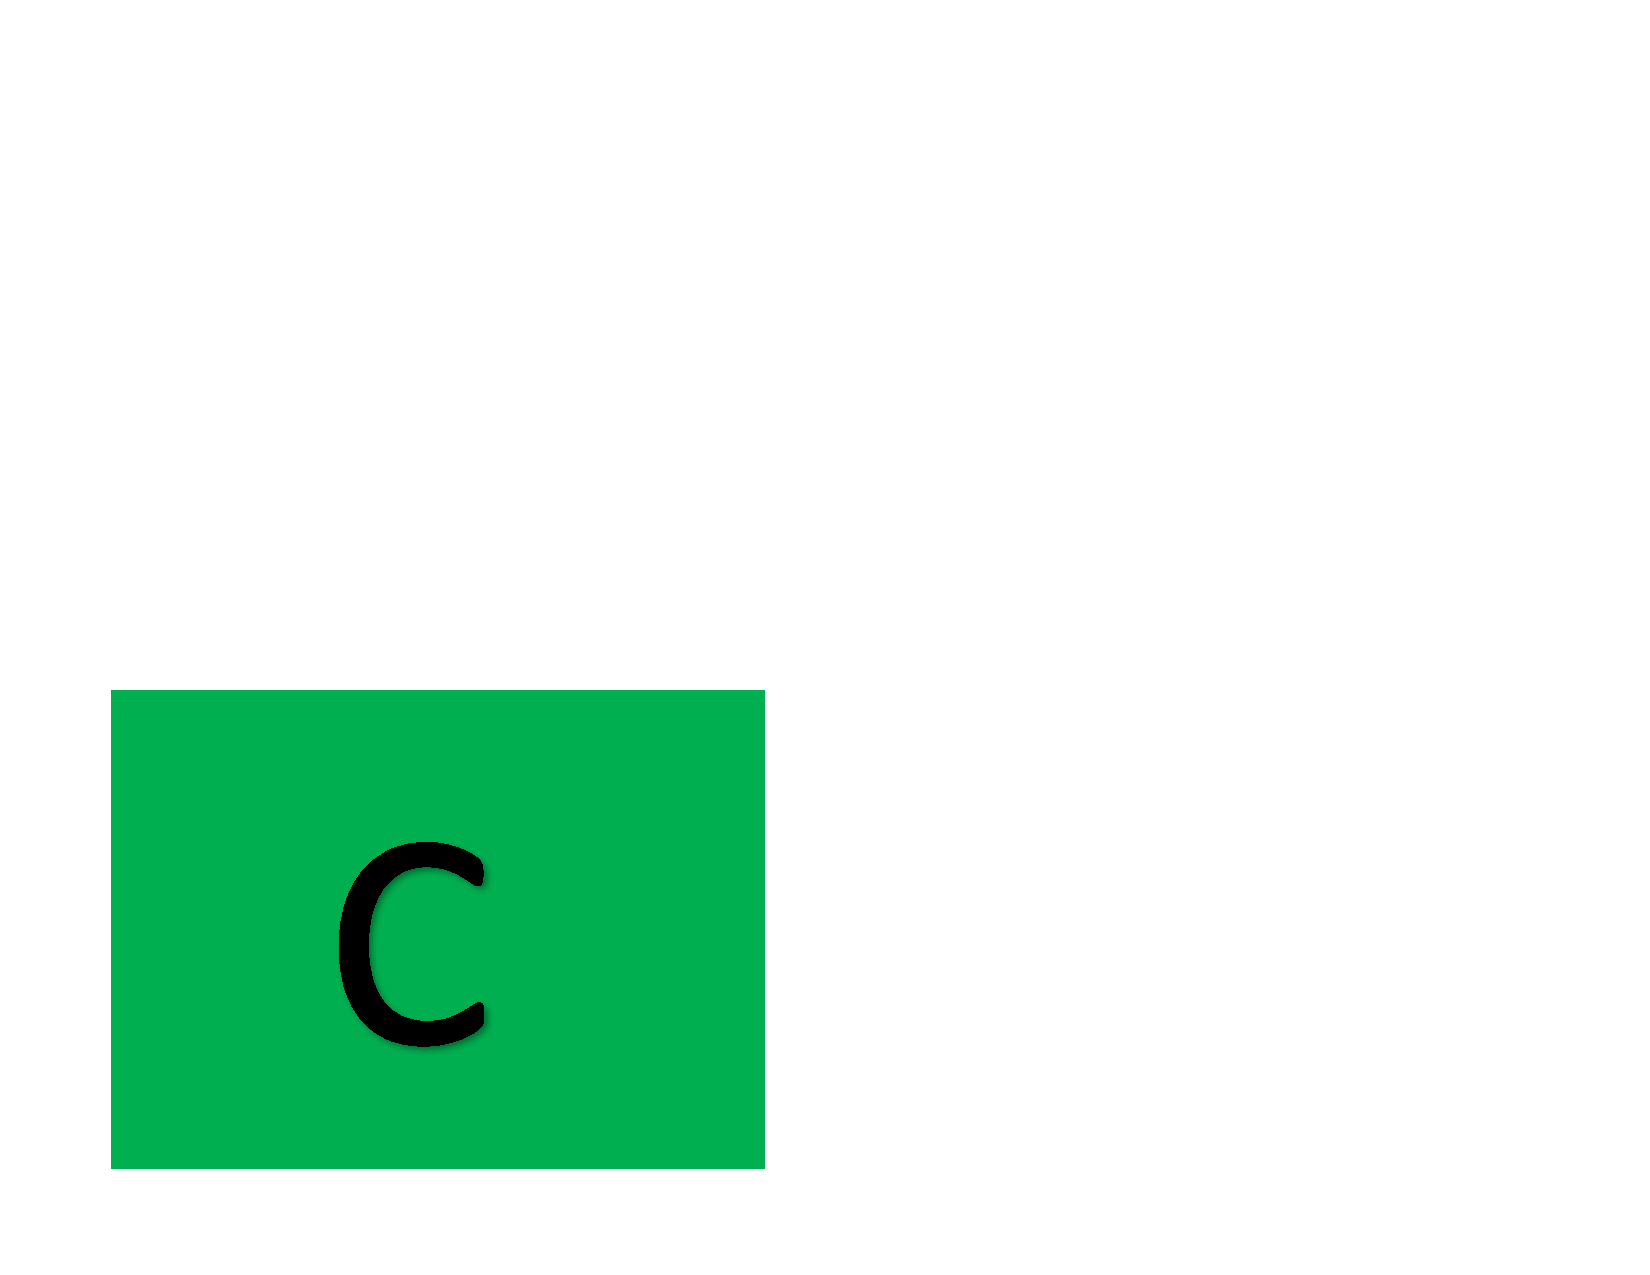
\includegraphics[width=0.8cm,height=0.5cm]{../../Lectures/figures/C}} ]  }
\newcommand*{\ditem}{ \item[{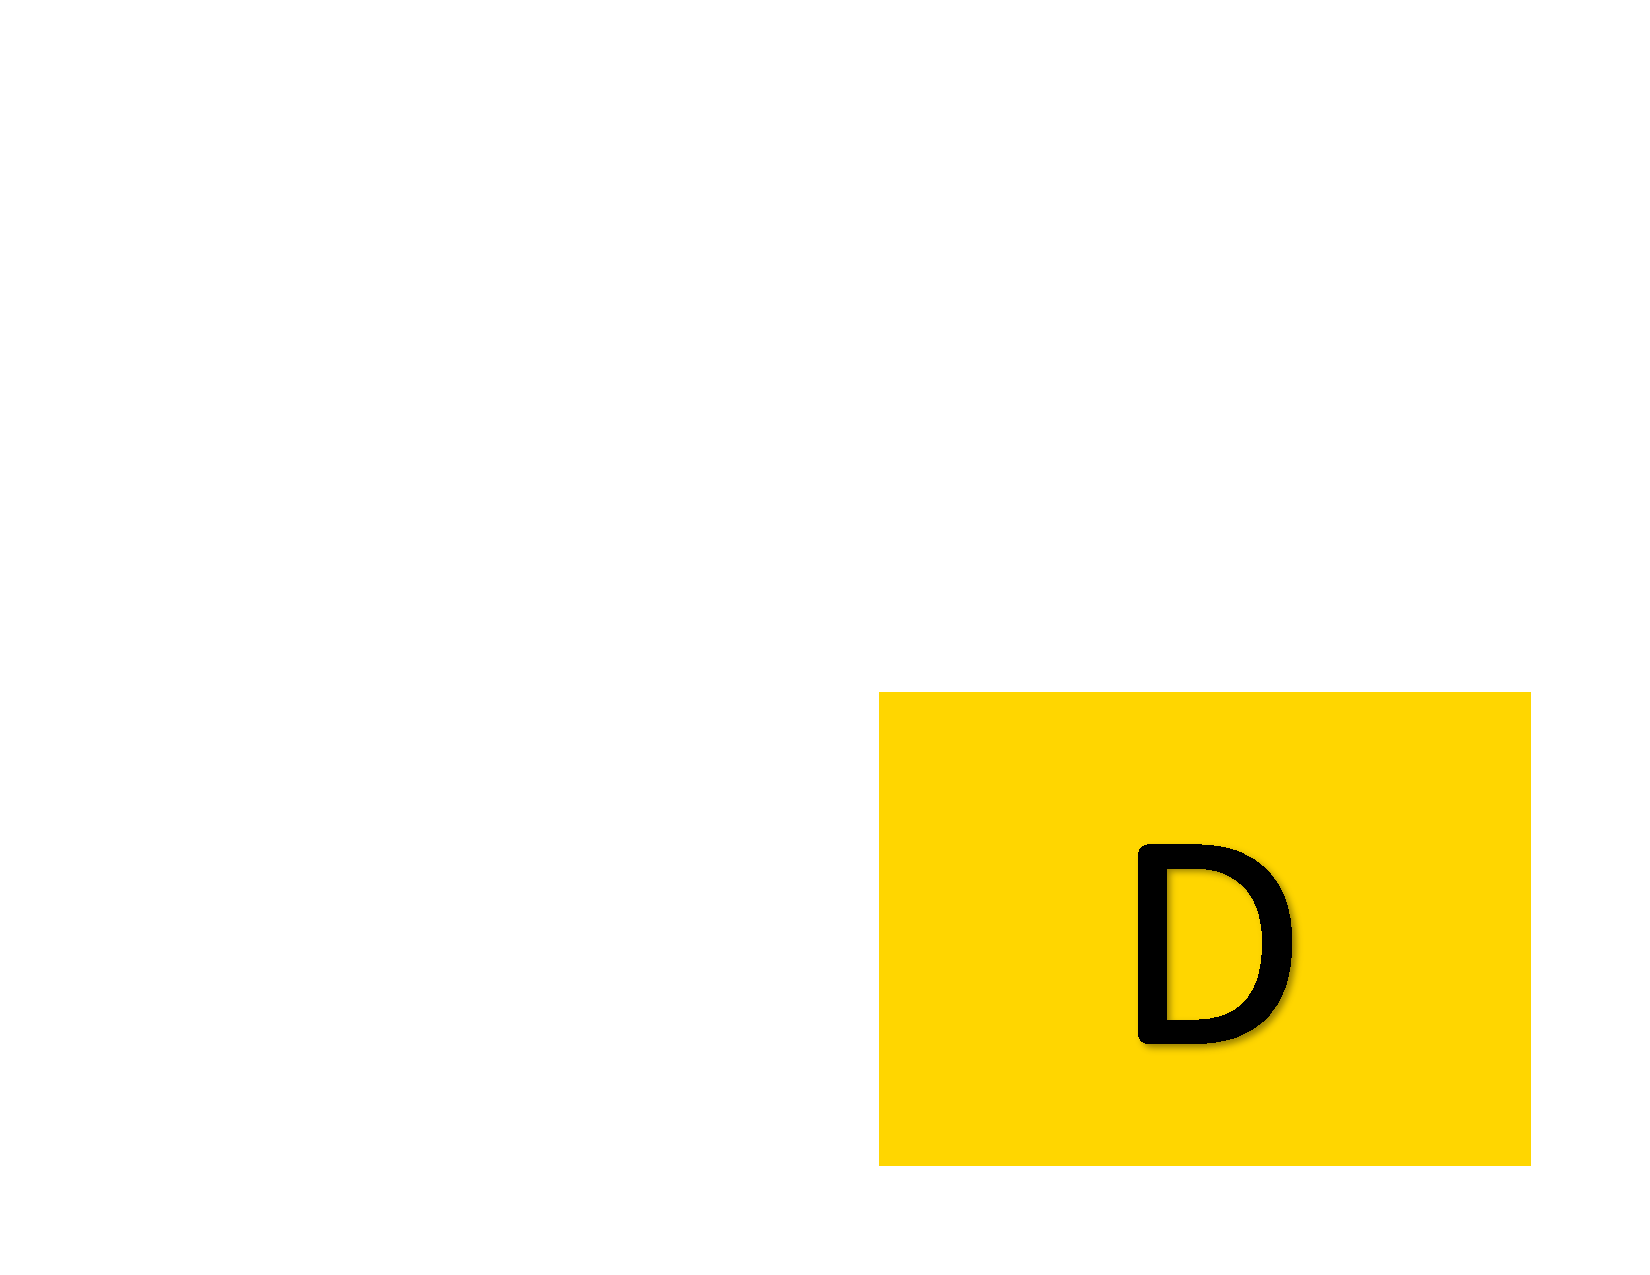
\includegraphics[width=0.8cm,height=0.5cm]{../../Lectures/figures/D}} ]  }
\newcommand*{\eitem}{ \item[{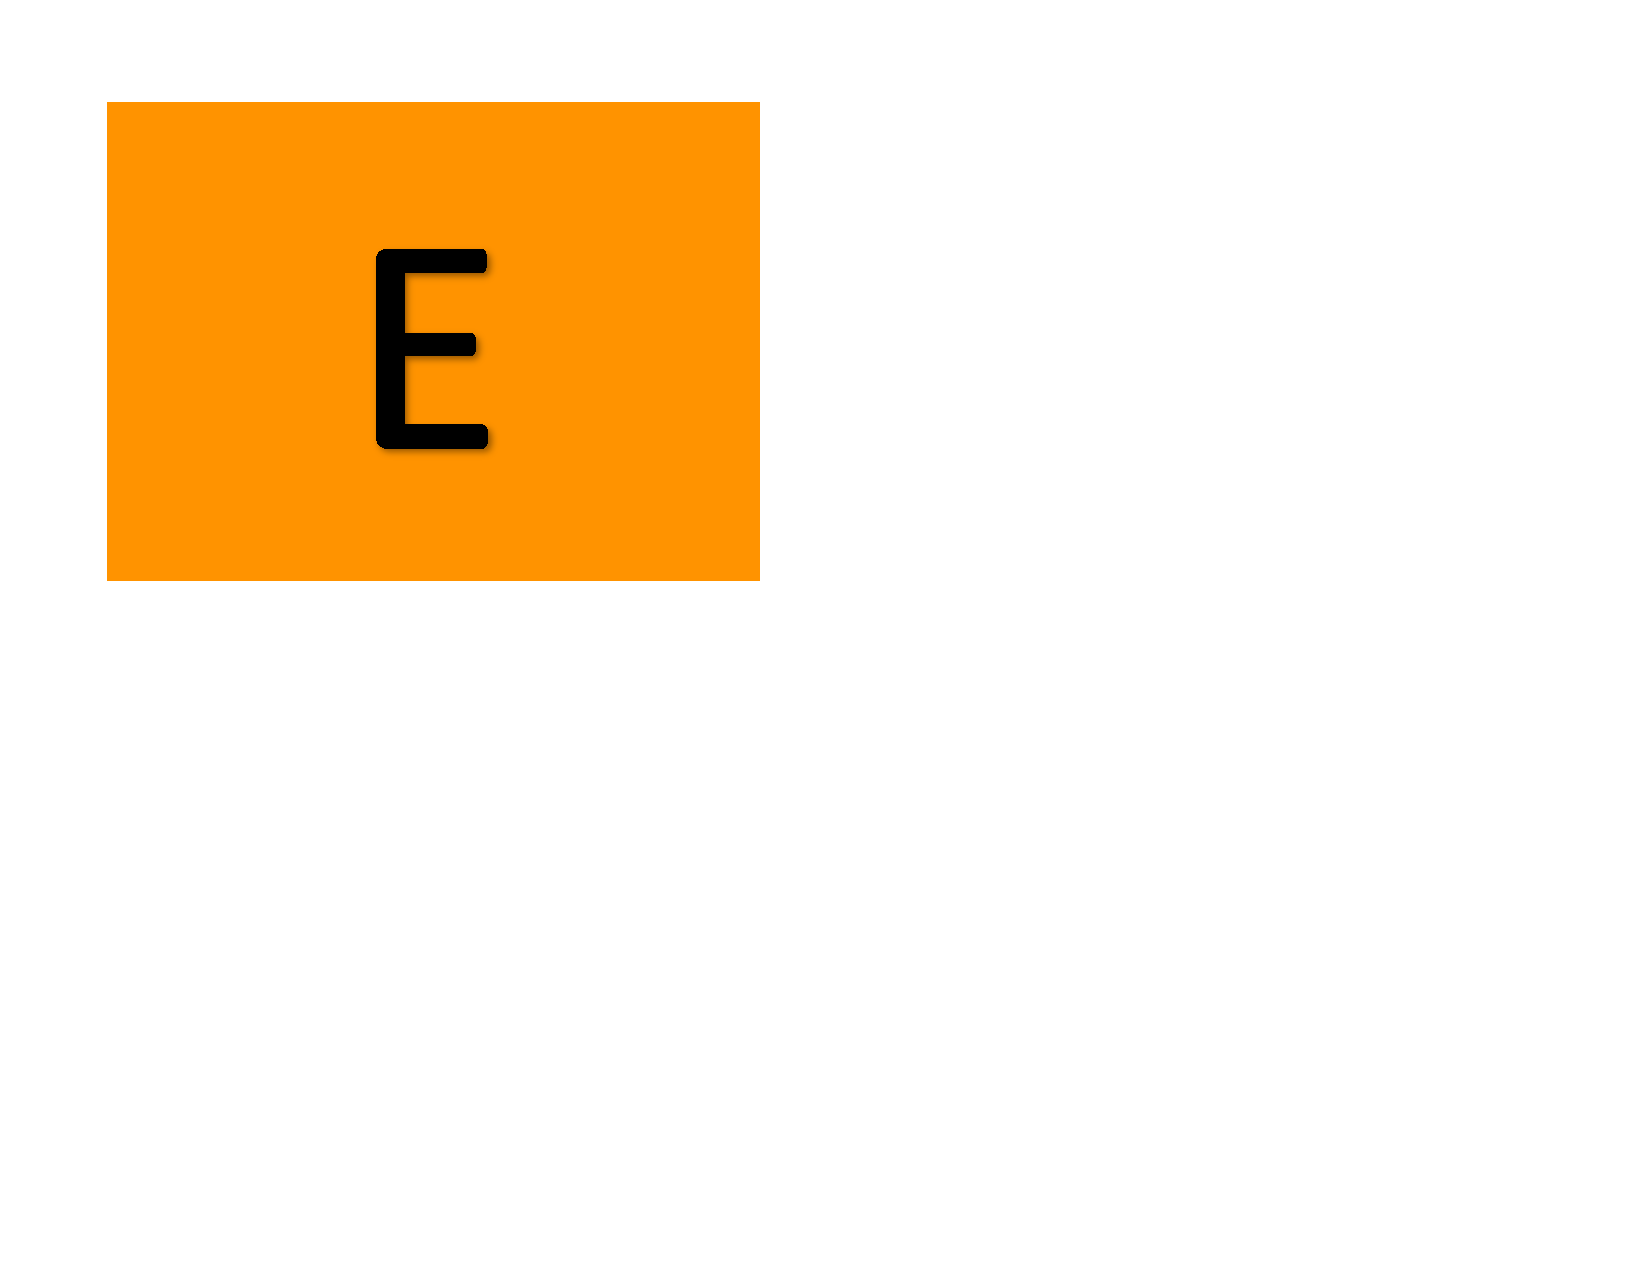
\includegraphics[width=0.8cm,height=0.5cm]{../../Lectures/figures/E}} ]  }
\newcommand*{\fitem}{ \item[{
\includegraphics[width=0.8cm,height=0.5cm]{../../Lectures/figures/F}} ]  }


\newcommand{\hide}[1]{\underline{\phantom{#1 #1}}}

\usepackage{setspace}

\onehalfspacing

\begin{document}
	
	
	\lecture{12: Graph Algorithms: DFS}{February 27}
	

	
	\section{Depth First Search Algorithm}
	Unlike in a BFS, a depth-first search (DFS):
	\begin{itemize}
		\item Explores the \emph{most recently discovered vertex} before backtracking and exploring other previously discovered vertices
		\item All nodes in the graph are explored (rather than just a DFS for a single node $s$)
		\item We keep track of a global \emph{time}, and each node is associated with two timestamps for when it is \emph{discovered} and \emph{explored}.
	\end{itemize}
	
	Each node $u \in V$ is associated with the following attributes
	
	\begin{tabular}{| l | p{8cm} | p{6cm} |}
		\hline
		Attribute & Explanation &Initialization \\
		\hline
		$u.\text{status}$ & tells us whether a node has been \emph{undiscovered}, \emph{discovered}, and \emph{explored} &  $u.\text{status} = U$\\
		\hline
		$u.\text{D}$ & timestamp when $u$ is first discovered & NIL  \\
		\hline
		$u.\text{F}$ & timestamp when $u$ is finished being explored   & NIL  \\
		\hline
		$u.\text{parent}$ & predecessor/``discoverer" of $u$ & NIL \\
		\hline
	\end{tabular}
	
	\vspace{1cm} 
	\begin{minipage}[t]{0.45\textwidth}
		%	\begin{algorithm}
		\textsc{DFS}($G$)
		\begin{algorithmic}
			\For{$v \in V $}
			\State $v.\text{parent} = NIL$
			\State $v.\text{status} = \text{U}$
			\EndFor
			\State $\text{time} = 0$
			\For{$u \in V$}
			\If{$u.\text{status} == U$}
			\State $\textsc{DFS-Visit}(G,u)$
			\EndIf
			\EndFor
		\end{algorithmic}
		%	\end{algorithm}
	\end{minipage}
	\begin{minipage}[t]{0.45\textwidth}
		%	\begin{algorithm}
		\textsc{DFS-Visit}($G,u$)
		\begin{algorithmic}
			\State $\text{time} = \text{time} + 1$
			\State $u.D = \text{time}$
			\State $u.\text{status} = D$
			\For{$v \in \text{Adj}[u]$}
			\If{$v.\text{status} == U$}
			\State $v.\text{parent} = u$
			\State $\textsc{DFS-Visit}(G,v)$
			\EndIf
			\EndFor
			\State $u.\text{status} = \text{E}$
			\State $\text{time} = \text{time} + 1$
			\State $u.F = \text{time}$
		\end{algorithmic}
		%	\end{algorithm}
	\end{minipage}
	\vspace{1cm}
	
	\newpage
	\subsection{Runtime Analysis}
	\begin{Qu}
		What is the runtime of a depth first search, assuming that we store the graph in an adjacency list, and assuming that $|E| = \Omega(|V|)$?
		\begin{itemize}
			\aitem $O(|V|)$
			\bitem $O(|E|)$
			\citem $O(|V| \times |E|)$
			\ditem $O(|V|^2)$
			\eitem $O(|E|^2)$
		\end{itemize}
	\end{Qu}
	\newpage
	\subsection{Properties of DFS}
	
	\begin{theorem}
		In any depth-first search of a graph $G = (V,E)$, for any pair of vertices $u$ and $v$, exactly one of the following conditions holds:\\ \\
		\begin{itemize}
			\item $[u.D,u.F]$ and $[v.D, v.F]$ are disjoint; \hide{neither of $u$ or $v$ is a} \\
			\item $[v.D, v.F]$ contains $[u.D,u.F]$ and \hide{$v$ is a descendant of $u$} \\
			\item $[u.D,u.F]$ contains $[v.D, v.F]$ and \hide{$u$ is a descendant of $v$}
		\end{itemize}
	\end{theorem}
	
	
	\textbf{We will not prove this, but we'll give a quick illustration}\\
	
		\begin{center}
	\includegraphics[width = .4\linewidth]{dfs.png}
\end{center}

\vspace{1cm} 
	\begin{center}
		{\Huge
	\begin{tabular}{|c |  c c c c c c c c c c c c |}
		\hline
		\textcircled{1} & 1 & 2 & 3 & 4 & 5 & 6 & 7 & 8 & 9 & 10 & 11 & 12 \\ \hline
		\textcircled{2} & 1 & 2 & 3 & 4 & 5 & 6 & 7 & 8 & 9 & 10 & 11 & 12 \\ \hline
		\textcircled{3} & 1 & 2 & 3 & 4 & 5 & 6 & 7 & 8 & 9 & 10 & 11 & 12 \\ \hline
		\textcircled{4} & 1 & 2 & 3 & 4 & 5 & 6 & 7 & 8 & 9 & 10 & 11 & 12 \\ \hline
		\textcircled{5} & 1 & 2 & 3 & 4 & 5 & 6 & 7 & 8 & 9 & 10 & 11 & 12 \\ \hline
		\textcircled{6} & 1 & 2 & 3 & 4 & 5 & 6 & 7 & 8 & 9 & 10 & 11 & 12 \\ \hline
	\end{tabular}
}
\end{center}
\vs{1cm}

\begin{corollary}
	$v$ is a descendant of $u \iff $ 
\end{corollary}

	\newpage
	\subsection{Classification of Edges}
	
	Given a graph $G = (V,E)$ performing a DFS on $G$ produces a graph $\hat{G} = (V, \hat{E})$ where
	\begin{align*}
		\hat{E} = \{ (u.\text{parent}, u) \colon v \in V \text{ and } v.\text{parent} \neq NIL  \}
	\end{align*}
	This is called a \emph{depth-first} forest of $G$. \\
	
	\vspace{4cm}
	
	Given any edge $(u,v) \in E$, we can classify it based on the status of node $v$ when we are performing the DFS:\\
	
	
	\begin{tabular}{| l | p{8cm} | p{6cm} |}
		\hline
		Edge & Explanation & How to tell when exploring $(u,v)$? \\
		\hline
		\textbf{Tree edge}  & edge in $\hat{E}$ & %$v.\text{status} == U$ 
		\\
		\hline
		\textbf{Back edge} & connects $u$ to ancestor $v$ & %$v.\text{status} == D$ 
		\\
		\hline
		\textbf{Forward edge} & connects vertex $u$ to descendant $v$ & \phantom{spaceasdfasdf2xsdf} \emph{and} $u.D < v.D$\\
		\hline
		\textbf{Cross edge} & either (a) connects two different trees or (b) crosses between siblings/cousins in same tree &  \phantom{spaceasdfasdf2xsdf} \emph{and} $u.D > v.D$\\
		\hline
	\end{tabular}
	

	\newpage
	\subsection{Practice}
	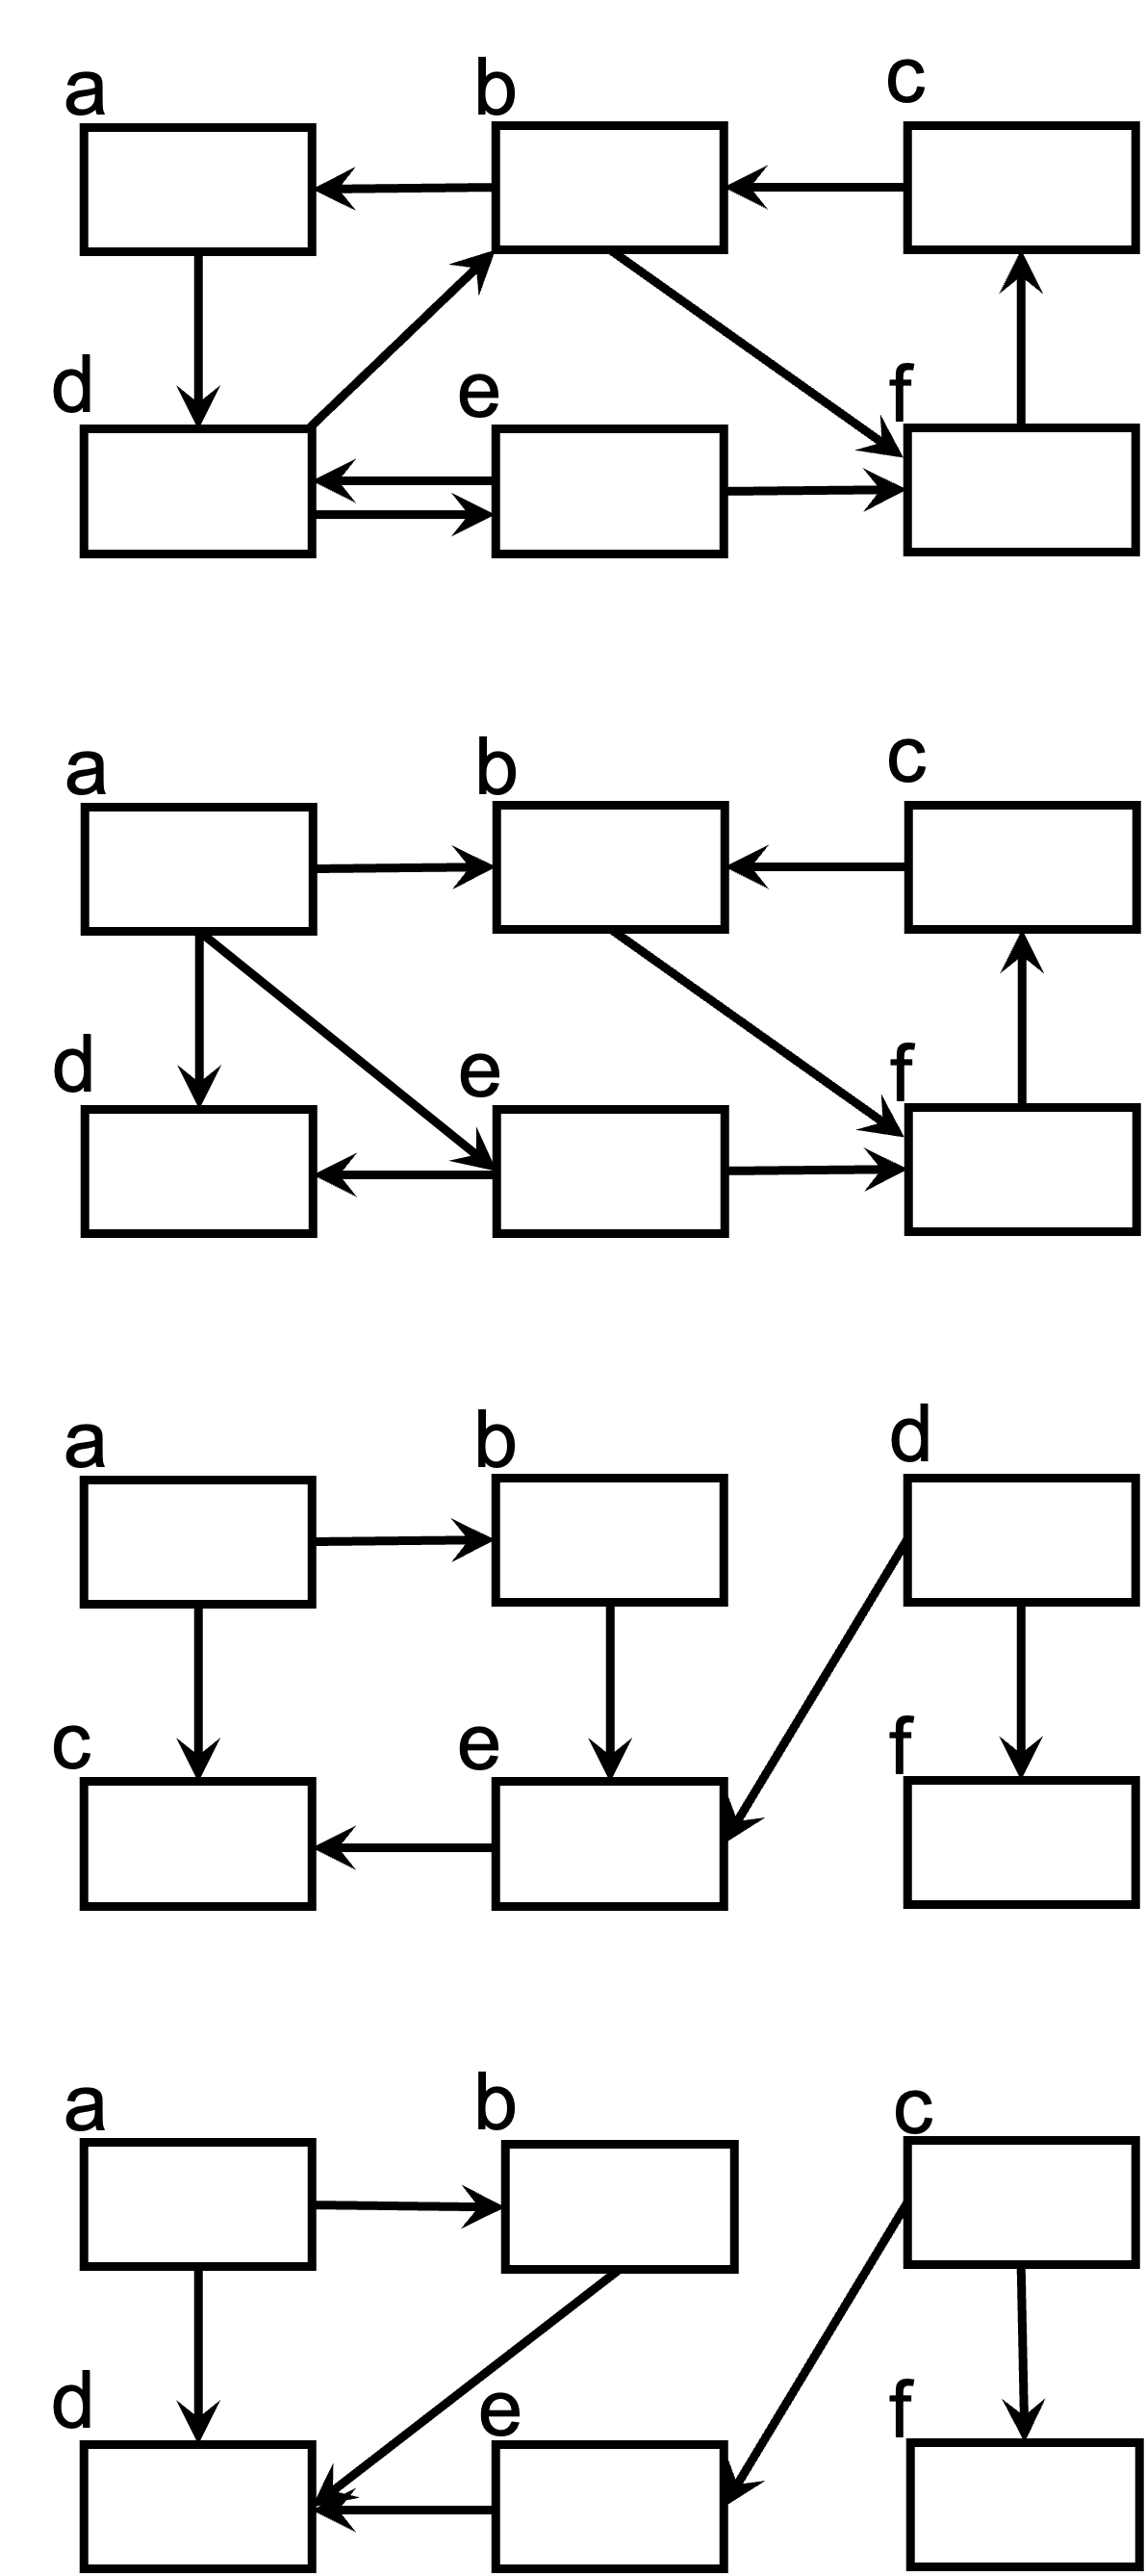
\includegraphics[width = .6\linewidth]{manydfs.png}
	\newpage
	\begin{Qu}
		How many of the above graphs were directed acyclic graphs?
		\begin{itemize}
			\aitem 1
			\bitem 2
			\citem 3
			\ditem 4
			\eitem none of them
		\end{itemize}
	\end{Qu}

\newpage

	\section{Application 1: Checking if $G$ is a DAG}
	
	\begin{theorem}
		$G$ is a DAG $\iff$ a DFS yields no back edges. Equivalently:
		\begin{center}
			\hide{A DFS yields a back edge $\iff$ $G$ is .}
		\end{center}
	\end{theorem}
	
	\textit{Proof} First, ($\implies$) we show that if DFS yields a back edge, $G$ is not a DAG.\\
	\vspace{4cm}
	
	
	Next ($\Leftarrow$) we show that if $G$ is not a DAG there will be a back edge.\\
	
	\newpage
	
	\section{Application 2: Topological Sort}
	Given a directed acyclic graph $G = (V,E)$, a topological sort of $G$ is an ordering of nodes such that for any $(u,v) \in E$, $u$ comes before $v$ in the ordering. \\
	
	We can use the following procedure to solve the topological sort problem:
	\begin{enumerate}
		\item  %Perform a DFS on $G = (V,E)$ \\
		\item  %Order nodes by reverse order of finish time (i.e., last node to be fully explored is the first node in the ordering)
		\vs{1cm}
	\end{enumerate}
	
	
	
	\newpage
	\begin{theorem}
		Ordering nodes in a directed acyclic graph $G = (V,E)$ by reversed finish times will produce a topological sort of $G$. 
	\end{theorem}
	\begin{proof}
		\begin{enumerate}
			\item Let $(u,v)$ be an edge in $G$
			\vs{2cm}
			\item Our goal is to show that 
			
			\begin{equation*}
				\hide{v.F < u.F}
			\end{equation*}
			
			\item When $(u,v)$ is explored, there are three different possibilities for the status of $v$:
			
			\begin{itemize}
				\item \textbf{Case 1}: $v.\text{status} == U$. This means $v$ becomes a descendant of $u$. \\
				
				Thus, $v.F < u.F$. Reason: \hide{Corollary 1.2}\\ \\
				
				\item \textbf{Case 2}: $v.\text{status} == E$, then we also have $v.F < u.F$.\\
				
				Reason:  \\ \\ 
				
				\item \textbf{Case 3}: $v.\text{status} == D$, this means that $v$ is an ancestor of $u$, so $(u,v)$ is a back edge. \\
				
				But this is impossible. Reason: \hide{Corollary 1.2}  \\ \\ \\
				
			\end{itemize}
			\item In all cases that are possible, \hide{$v.F < u.F$.}
		\end{enumerate}
		
		
	\end{proof}
	
	
\end{document}


\newpage
